% ============================================================
\chapter{A1: Discovering the Graph}
\label{chap:discovery}
% ============================================================

This chapter presents the discovery pipeline (A1, addressing C1) that produces
the object at the centre of Q: a credible, reproducible asset--asset causal
graph at every monthly rebalance of the 2007--2024 backtest.
Section~\ref{sec:data} describes the data; Section~\ref{sec:discovery-run} the
rolling discovery, the directional prior, and its empirical verification;
Section~\ref{sec:asset-graph} the extraction chokepoint through which every
allocator receives the identical graph, and what those graphs look like;
Section~\ref{sec:comparators} the two comparator graphs;
Section~\ref{sec:selection} the driver-selection arm retained from the
project's starting framework; and Section~\ref{sec:cache} the engineering that
makes the whole programme tractable and bit-reproducible.

\section{Data layer}
\label{sec:data}

\paragraph{Universe.} The target scale is the S\&P~100: large enough to be
representative, small enough that discovery at every rebalance remains
sweepable (fit cost grows steeply with dimension;
Section~\ref{sec:cache}). Official historical S\&P~100 membership is
paywalled and cannot be reconstructed from S\&P~500 records --- the index is
chosen with undisclosed sector-balance discretion --- so the standard
academic substitute is used: the top names by CRSP market capitalisation
among historical S\&P~500 members at each rebalance, whose union across
rebalances gives a fixed 99-asset universe over 2007--2024. Prices and
point-in-time shares outstanding come from WRDS/CRSP, which includes names
that later delisted --- essential for an honest 2008--09, when several dozen
large-cap financials disappeared --- with a thin Yahoo Finance fallback for
the most recent days. Late-inception names (post-2007 listings and merger
successors) are retained via a per-date eligibility mask rather than by
truncating every other series' history. The top-by-market-cap construction
remains an approximation of the official index and is noted as a limitation
in Section~\ref{sec:limitations}.

\paragraph{Driver pool.} Discovery runs on the \emph{joint} panel of assets
and 33 plausibly exogenous macro-financial series from FRED and Yahoo Finance:
Treasury rates and slopes, credit spreads, commodities, FX pairs, volatility
indices, and international-equity ETFs. The drivers serve two purposes: they
are the selection pool for the driver route (Section~\ref{sec:driver-route}),
and --- more importantly for Q --- their presence in the joint fit means the
asset--asset block is estimated \emph{conditional on} the common macro
environment, absorbing driver-explained co-movement that would otherwise
masquerade as asset-to-asset edges. Series that fail exogeneity to a US
large-cap portfolio --- sector ETFs, US index returns, factor portfolios ---
are excluded from the pool.

\paragraph{Stationarity and transforms.} SVAR-based discovery assumes weakly
stationary inputs. Each series is transformed \emph{by type}: log-returns for
price-like series; first differences for yields and spreads, which cross zero,
so logs are undefined; year-on-year changes for monthly macro levels, which
also removes seasonality; level pass-through for the already-stationary
volatility indices. A uniform ``log everything'' rule would break on the
rates block. The per-type transforms are fixed \emph{a priori} rather than
chosen by test per window, so each variable means the same thing in every
rolling window --- a prerequisite for comparing graphs across time.
Stationarity is then checked with both ADF and KPSS --- complementary because
their nulls are opposite, so agreement is a stronger signal than either alone
--- and failures are flagged and logged rather than used to drop series.

\section{Rolling discovery and the directional prior}
\label{sec:discovery-run}

The primary discovery method is chosen against three requirements, not by
default: it must scale to the ${\sim}132$-variable joint panel at every
rebalance of a sweepable grid; it must accept the directional prior of C1
\emph{natively}, rather than by post-hoc edge deletion; and it must return a
genuine DAG, because the allocators of Chapter~\ref{chap:sensitivity} rely
on exact nilpotent total-effect algebra. DYNOTEARS meets all three; the
comparators of Section~\ref{sec:comparators} each relax one requirement and
so double as probes of whether the requirement mattered.

At each rebalance date $t$, DYNOTEARS \cite{pamfil2020dynotears} is fit on the
per-window $z$-scored joint panel $X=[\,D \mid A\,]$ over the lookback window
(252 or 504 trading days), with lag $p=1$ --- lagged structure beyond one
step is negligible at these horizons (Section~\ref{sec:howard-theme}) ---
yielding the contemporaneous matrix
$W$ (acyclicity enforced) and lagged matrix $A_1$ over the joint variable set.
The convention throughout is $M[i,j]$ = effect of variable $i$ on variable
$j$; the operative hyperparameters are tabulated in
Appendix~\ref{app:tables}.

\paragraph{Enforcing the prior.} The directional prior of C1 --- drivers may
cause assets; individual large-cap stocks do not cause the 10-year Treasury
yield at these scales --- is enforced natively: DYNOTEARS accepts a forbidden-
edge list (\texttt{tabu\_edges}), populated with every asset$\to$driver pair
at every lag, forcing those entries of $W$ and $A_1$ to zero. VARLiNGAM
enforces the same prior through its prior-knowledge mechanism plus a post-fit
projection.

\paragraph{Does the prior matter? (verification).} A prior is only worth its
place if it does real work. Refitting DYNOTEARS with and without the prior on
six windows spanning distinct regimes (2008, 2011, 2014, 2018Q4, 2020, 2022)
shows that, unconstrained, the optimiser spends \textbf{35--48\%} of total
edge mass on economically implausible asset$\to$driver edges; admitting them
distorts the legitimate driver$\to$asset block by 52--72\% in $L_1$ and
shifts the selected driver set in a meaningful minority of windows (top-$K$
Jaccard 0.62--1.00, lowest in the 2008 and 2022 stress regimes;
Figure~\ref{fig:prior}). The prior is consequential, not cosmetic --- it
cheaply removes a large block of spurious reverse-causation mass --- and,
because the asset--asset block is estimated jointly, it protects the graph
that Q's allocators consume.

\begin{figure}[tbp]
  \centering
  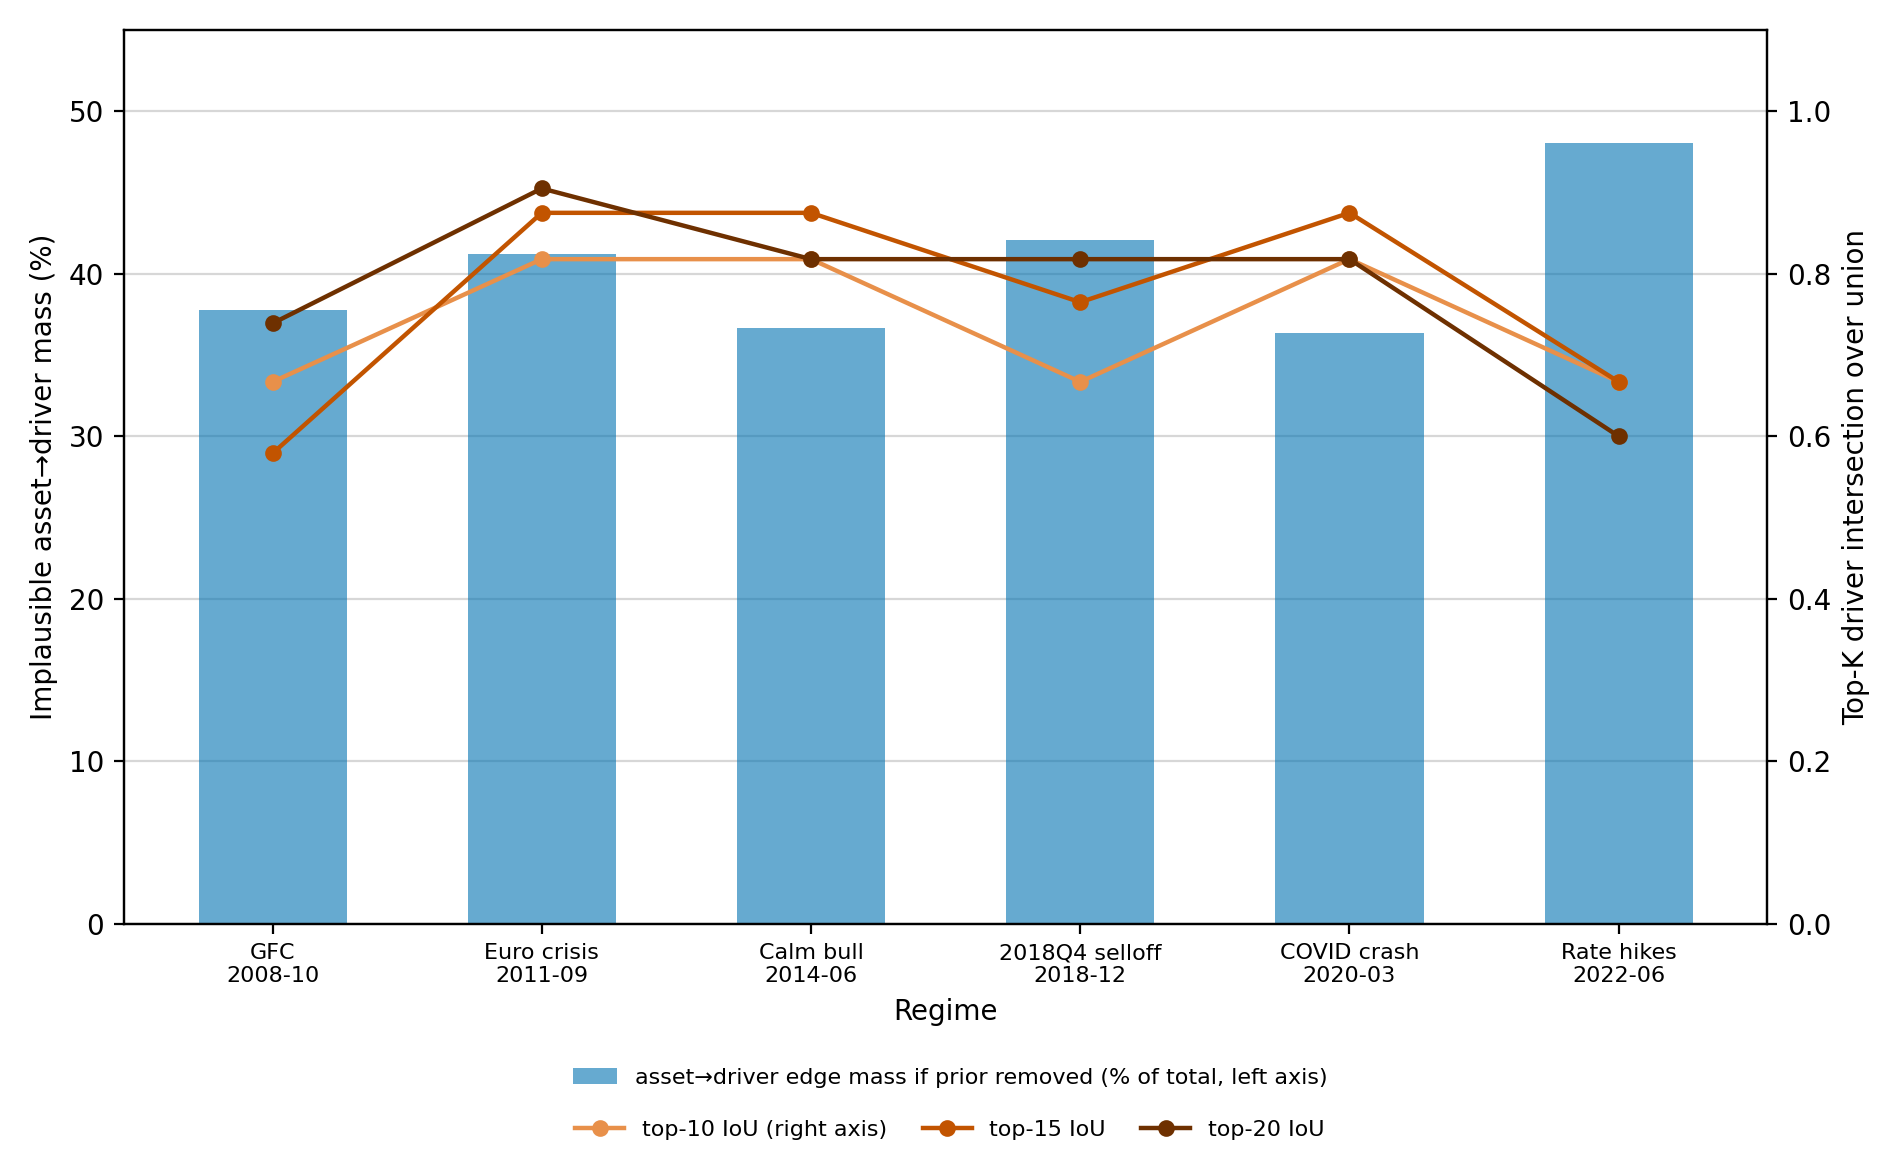
\includegraphics[width=0.92\textwidth]{figures/directional_prior.png}
  \caption{Verification of the asset$\to$driver directional prior. Bars: the
    fraction of total DYNOTEARS edge mass that would fall on implausible
    asset$\to$driver edges if the prior were removed (35--48\% across regime
    windows). Line (right axis): top-$K$ driver-set Jaccard with versus
    without the prior. The prior removes a large block of spurious
    reverse-causation mass, and matters most in the 2008 and 2022 stress
    regimes.}
  \label{fig:prior}
\end{figure}

\section{The asset-graph chokepoint}
\label{sec:asset-graph}

Q's fixed-graph ablation is only valid if every allocator sees the
\emph{byte-identical} graph, so extraction is centralised in a single
chokepoint rather than left to each allocator. Per rebalance it reads the
asset--asset block $M$ of the fitted contemporaneous matrix; restricts rows
\emph{and} columns together to the eligible universe at that date (so
late-inception names can never desynchronise the graph from the returns
panel); applies the magnitude threshold $\tau$ (default $0$; swept in the
sparsity-robustness analysis); and verifies acyclicity (a sub-block of a DAG
is a DAG). It also computes the per-asset structural residual variances on
the fit window --- needed by the structural covariance of
Section~\ref{sec:d-family} --- using the window's stored $z$-statistics, so
the residuals correspond exactly to the data the graph was fitted on.

\paragraph{What the graphs look like.} The DAGs are far from degenerate,
and stably so across estimation horizons: at every window from 189 to 504
days the DYNOTEARS asset graphs average ${\sim}615$--$655$ directed edges
(density $6.3$--$6.7\%$ of possible ordered pairs) with a longest directed
path of ${\approx}50$ nodes out of 99 --- deep chains of influence, not a
shallow hub-and-spoke. There is, in other words, substantial orientation
structure for the treatment allocators to exploit; whatever the evaluation
finds, it will not be because the graphs were trivially symmetric. (The
same diagnostic flags a comparator limitation: VARLiNGAM's unpruned $B_0$
saturates to $32\%$ density at the 189-day window --- $n=189$ observations
against $d=132$ variables --- where DYNOTEARS' $\ell_1$ objective holds
density steady.)

\paragraph{What ``credible'' can mean without ground truth.} An objection
must be met head-on: no true causal graph of the market is available, so the
discovered graphs cannot be scored against an answer key. The pipeline is
therefore validated on everything that \emph{can} be checked: the
directional prior does real, quantified work (above); the graphs are
structurally non-degenerate, with genuine depth for the treatments to
exploit; discovery is deterministic, so the graphs are at least stable
facts about the data rather than artefacts of a run; disagreement between
discovery methods is retained as a diagnostic rather than averaged away
(Section~\ref{sec:comparators}); and, decisively, the graphs are judged by
the controlled downstream ablation of
Chapters~\ref{chap:sensitivity}--\ref{chap:evaluation} --- a task-based
test, which is the only economically meaningful one. The report accordingly
claims that the graphs are \emph{useful and reproducible}, never that they
are \emph{true}.

\section{Comparator graphs}
\label{sec:comparators}

Two further graph sources feed the same chokepoint, so every allocator runs
unchanged on them. \textbf{VARLiNGAM} \cite{hyvarinen2010varlingam} supplies
the instantaneous matrix $B_0$, identified through non-Gaussianity rather
than a score: LiNGAM's causal order makes the asset block a DAG by
construction, and its identification assumption --- heavy-tailed residuals ---
weakens mechanically at longer windows, the window-fragility
Chapter~\ref{chap:background} anticipated and Chapter~\ref{chap:evaluation}
observes. \textbf{GRANGER} is the deliberately cheap comparator: a
ridge-regularised VAR(1) on the asset panel, in closed form, with
$M[i,j] = |{\rm coef}(x_{i,t-1}\!\to\!x_{j,t})|$, thresholded per window
to match the paired DYNOTEARS graph's edge density so the comparison is at
like-for-like sparsity. It is deterministic and assumption-light, but its
matrix is lagged rather than contemporaneous and is not guaranteed acyclic;
the allocators handle this honestly (truncated-Neumann total effects; minimal
feedback-arc removal before topological ordering). If GRANGER allocates as
well as DYNOTEARS, expensive discovery is not where the value lies. (A
non-linear extension, NTS-NOTEARS \cite{sun2023ntsnotears}, was probed at
reduced scale: its prior-knowledge mechanism drives the asset$\to$driver
block to exactly zero and its discovered structure agrees with DYNOTEARS only
modestly --- a genuinely different lens --- but at ${\sim}10\times$ the fit
cost a full backtest is future work.)

\section{The driver-selection arm}
\label{sec:selection}

The project's starting framework (HSP) needs $K$ drivers selected per
rebalance; the arm is retained as a supporting comparison
(Section~\ref{sec:driver-route}), so its mechanics are summarised. Selection
is two-stage on the discovered graph: Stage~A scores each driver by its
aggregate outgoing influence on the assets and shortlists; Stage~B adds
drivers greedily by marginal held-out predictive gain. The count $K$ is
calibrated once on a burn-in window by the Kneedle elbow
\cite{satopaa2011kneedle} ($K=17$ at full scale), alongside a permutation
null with Benjamini--Hochberg FDR control \cite{benjamini1995fdr} --- which
returns the honest answer that \emph{zero} drivers clear 5\% significance
against shuffled data: the per-driver causal signal at this universe size is
weak, a caveat that foreshadows the arm's evaluation. Qualitatively the
causal selector still does what the correlation selector cannot --- it
rotates across ${\sim}26$ regime-tracking drivers where cumulative
correlation locks onto the same international-equity ETFs and rates-curve
points at essentially every rebalance --- but Q does not rest on this arm.

\section{Engineering for tractability and reproducibility}
\label{sec:cache}

Two engineering results underwrite the credibility of every number in
Chapter~\ref{chap:evaluation}.

\paragraph{The discovery cache.} The graph fit is the dominant cost
(${\approx}4$ minutes per window at $d\approx132$; ${\approx}15$ hours per
215-rebalance backtest), yet it depends only on the window data and discovery
hyperparameters --- not on anything downstream. A content-keyed disk cache
(keyed by the exact window bytes, column set, method and hyperparameters,
with atomic writes) therefore lets every configuration at a given window
reuse one fit. The effect is decisive for Q: the entire fixed-graph ablation
--- 56 allocator--method--window cells, plus sparsity, cost and comparator
sweeps --- ran against 1{,}684 cached graph fits with a verified 100\% hit
rate and zero refits (a key miss halts the run rather than silently
refitting a subtly different graph), at ${\approx}40$ seconds per backtest
instead of ${\approx}15$ hours; extending the window grid from two to four
horizons cost one overnight populate run rather than weeks. The cache is also what \emph{guarantees} the ablation's
premise: allocators cannot see different graphs, because there is exactly one
graph per (method, window, data) key.

\paragraph{A data-determinism defect, found and fixed.} Building the cache
exposed a latent reproducibility bug: one driver series (the
emerging-markets ETF EEM) was silently re-downloaded on every call because
its 2003 inception fell inside the cache-coverage check's padding window,
and auto-adjustment jittered its values by ${\approx}3\times10^{-7}$
run-to-run --- which the non-convex DYNOTEARS optimiser amplified into graph
changes of ${\approx}0.14$ in $\lVert W\rVert$. The pipeline was, in other
words, not bit-reproducible, and two previously-drawn conclusions (an
apparent two-year edge for causal driver selection, and an apparently
significantly-worse closed loop) did not survive the fix. The same fix left
the VARLiNGAM graphs essentially unchanged --- ICA on VAR residuals is far
less sensitive to input micro-jitter than non-convex L-BFGS, a small
robustness result in its own right. All numbers in this report come from the
corrected, deterministic pipeline: two independent runs now produce
byte-identical windows, weights and NAVs --- verified end-to-end by the
replication gate of Section~\ref{sec:ablation-design}. A result that does not
survive a determinism fix was never real; treating reproducibility as a
prerequisite rather than an afterthought is part of the method
\cite{lopezdeprado2023causal}.
